% !TeX program = pdflatex
\documentclass[11pt,a4paper]{article}

% Essential packages
\usepackage[utf8]{inputenc}
\usepackage[T1]{fontenc}
\usepackage{amsmath}
\usepackage{amsfonts}
\usepackage{amssymb}
\usepackage{graphicx}
\usepackage{hyperref}
\usepackage{geometry}
\usepackage{setspace}
\usepackage{booktabs}
\usepackage{float}
\usepackage{cleveref}
\usepackage{titling}
\usepackage{tikz}
\usetikzlibrary{shapes,arrows,positioning}

% Page layout
\geometry{
    a4paper,
    margin=2.5cm
}

% Hyperref settings
\hypersetup{
    colorlinks=true,
    linkcolor=blue,
    filecolor=magenta,
    urlcolor=cyan,
    citecolor=blue
}

% Document info
\title{Songjam\\[0.5em]\large A Cryptographic Voice Verification System}
\author{Adam Place}
\date{\today}

% Customize title formatting
\pretitle{\begin{center}\LARGE\bfseries}
\posttitle{\par\end{center}}

\begin{document}

\maketitle

\begin{abstract}
The proliferation of deepfake technology has exposed critical vulnerabilities in voice-based authentication, leading to high-profile financial losses and widespread consumer fraud. Existing real-time detection methods are constrained by technical and privacy limitations, especially in proprietary communication platforms. This paper introduces a privacy-preserving, cryptoeconomic framework for secure voice verification, leveraging zero-knowledge proofs and selective disclosure to authenticate participants without exposing sensitive data. Inspired by the economic incentives and penalties of Proof-of-Stake (PoS) consensus mechanisms, this approach incentivizes accurate credential provision and penalizes fraudulent behavior, aligning security with compliance. The efficacy of this model is analysed in mitigating deepfake threats and discuss its practical deployment within enterprise and consumer communication networks.
\end{abstract}

\section{Introduction}
\label{sec:introduction}
The rise of deepfakes has led to a growing concern about the falibility of humans to verify the authenticity of voice communication.
High profile cases such as the 2024 deepfake attack on engineering firm Arup, which led to a twenty-five million dollar loss, highlight the importance of secure and reliable enterprise verification systems.

While a plethora of fradulent online videos featuring deepfakes of celebrities promoting supposed investment opportunities, and the rise of romance or 'pig butchering' scams which collectively siphon billions of dollars from unsuspecting victims every year illustrate the nessecity of consumer or citizen protections.
The sub-150ms latency required for natural conversation in VoIP calls leaves minimal time for analysis on standard hardware, making real-time detection of deepfakes challenging. While the proprietary nature of platforms such as Zoom, Teams and SIP providers, hinders the development of universal detection frameworks.

What is needed is a privacy-preserving verification system leveraging zero-knowledge proofs and selective disclosure mechanisms, where only cryptographically attested credentials (e.g., identity, access rights) are validated—without exposing extraneous user data.
This approach ensures networks authenticate voice participants a priori through mathematical guarantees (e.g., zk-SNARKs), verifying the existence of valid credentials rather than analyzing raw biometrics or personal details.
By limiting verification to key attributes (e.g., "member of authorised group" or "registered device") and eliminating unnecessary data collection, such systems align with GDPR/CCPA principles while thwarting deepfake fraud and metadata misuse.
This paper proposes a novel cryptoeconomic framework for voice verification, in which users are incentivised to provide accurate and verifiable credentials, while malicious actors face penalties—akin to Proof-of-Stake slashing mechanisms—for fraudulent voice attribution attempts.

\section{The Proof-of-Stake Security Guarentee?}
\label{sec:background}
Much has been written about the security of the Proof-of-Stake (PoS) consensus mechanism, with proponents arguing that its economic incentives guarantee security, while opponents contend that the consolidation of staked token supply will lead to centralisation.
Nevertheless, the economic incentives and penalties underpinning Ethereum’s Proof-of-Stake mechanism have proven effective, driving its adoption and establishing it as the preferred consensus model for securing one of the world’s largest blockchain networks—demonstrated by the very small number of validator slashing events recorded to date (with only around 0.045\% of validators slashed since Ethereum staking began).

\begin{figure}[h]
    \centering
    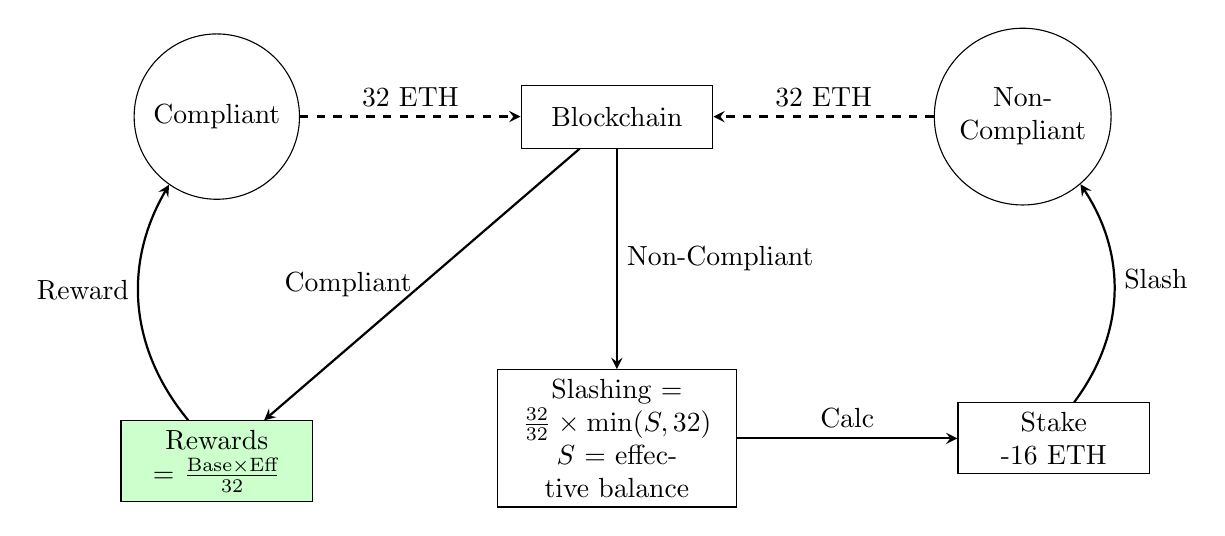
\begin{tikzpicture}[
        node distance=2.8cm,
        block/.style={rectangle, draw, text width=2.2cm, text centered, minimum height=0.8cm},
        validator/.style={circle, draw, text width=1.8cm, text centered, minimum height=0.8cm},
        arrow/.style={thick,->,>=stealth},
        dashedarrow/.style={thick,dashed,->,>=stealth},
        math/.style={rectangle, draw, text width=2.8cm, text centered, minimum height=1.2cm},
        reward/.style={rectangle, draw, text width=2.2cm, text centered, minimum height=0.8cm, fill=green!20}
    ]
        % Blockchain
        \node[block] (blockchain) {Blockchain};
        
        % Validators - using larger distances
        \node[validator, left=2.8cm of blockchain] (validator1) {Compliant};
        \node[validator, right=2.8cm of blockchain] (validator2) {Non-Compliant};
        
        % Staking connections
        \draw[dashedarrow] (validator1) -- node[above] {32 ETH} (blockchain);
        \draw[dashedarrow] (validator2) -- node[above] {32 ETH} (blockchain);
        
        % Slashing penalty
        \node[math, below=of blockchain] (penalties) {
            Slashing = $\frac{32}{32} \times \text{min}(S, 32)$\\
            $S$ = effective balance
        };
        
        % Stake reduction
        \node[block, right=of penalties] (reduction) {Stake -16 ETH};
        
        % Rewards
        \node[reward, below=of validator1] (rewards) {
            Rewards = $\frac{\text{Base} \times \text{Eff}}{32}$
        };
        
        % Connections
        \draw[arrow] (blockchain) -- node[right] {Non-Compliant} (penalties);
        \draw[arrow] (penalties) -- node[above] {Calc} (reduction);
        \draw[arrow] (reduction) to[bend right=35] node[right, yshift=0.2cm] {Slash} (validator2);
        \draw[arrow] (blockchain) -- node[left] {Compliant} (rewards);
        \draw[arrow] (rewards) to[bend left=35] node[left, yshift=0.2cm] {Reward} (validator1);
    \end{tikzpicture}
    \caption{Ethereum's PoS economics rewards honest validators and penalises malicious ones}
    \label{fig:pos-system}
\end{figure}



\section{Soulbound Tokens}
\label{sec:methodology}
Describe your methods and approach here.

\section{Voice Biometrics}
\label{sec:results}
Present your results here.

\section{AI Voice Agents}
\label{sec:discussion}
Discuss your findings and their implications here.

\section{Conclusion}
\label{sec:conclusion}
Conclude your paper here.

\bibliographystyle{plain}
\bibliography{references}

\end{document} 